\chapter{Layer Sweeps}
\label{chap:appendix-layer-sweeps}

This appendix reports the out-of-fold probe accuracy by layer, against the coordinator's flat accuracy, for each of the eight models of Chapter~\ref{chap:probing-results}, on the single-turn and the multi-turn dataset. Each model's optimal layer, read off these sweeps, is reported in its table in Section~\ref{sec:ch7-results}.

\section{Gemma 4 E2B IT}
\label{sec:appendix-layer-sweep-gemma4-e2b-it}

\begin{figure}[H]
    \centering
    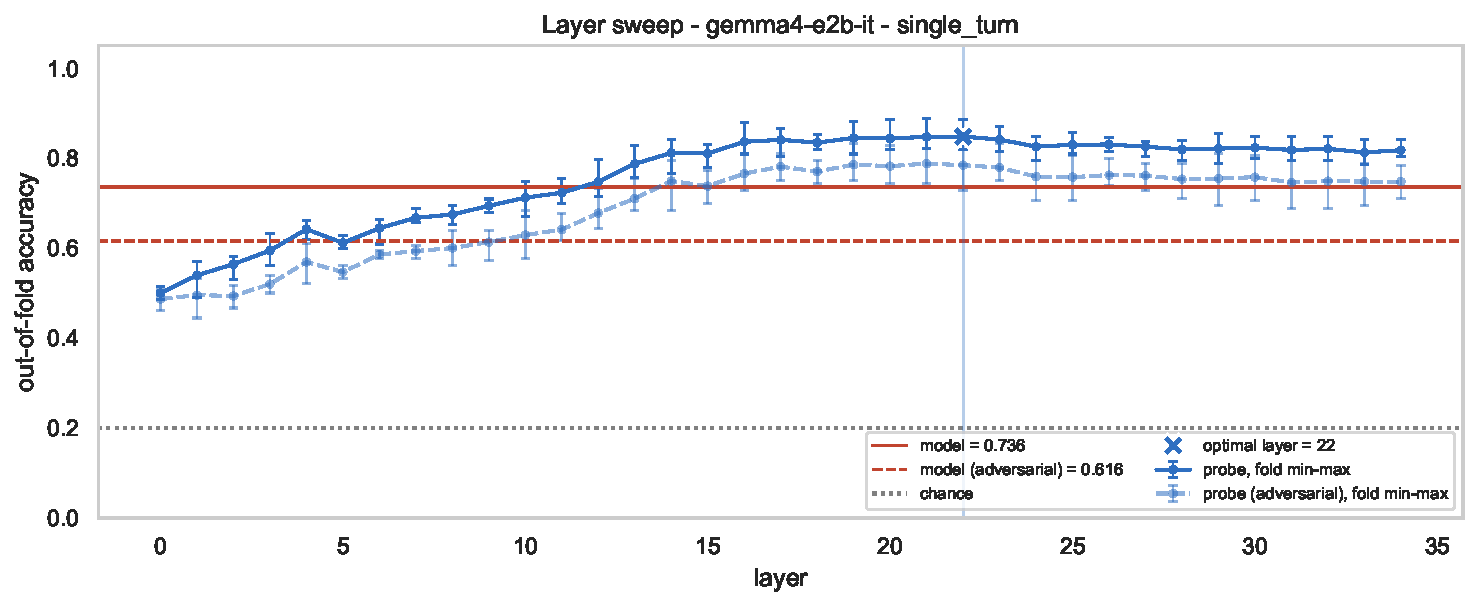
\includegraphics[width=0.85\textwidth]{images/models/gemma4-e2b-it_single_turn_layers.pdf}
    \caption[Layer sweep, gemma4-e2b-it, single-turn]{Layer sweep, gemma4-e2b-it, single-turn.}
    \label{fig:appendix-gemma4-e2b-it-single-layers}
\end{figure}

\begin{figure}[H]
    \centering
    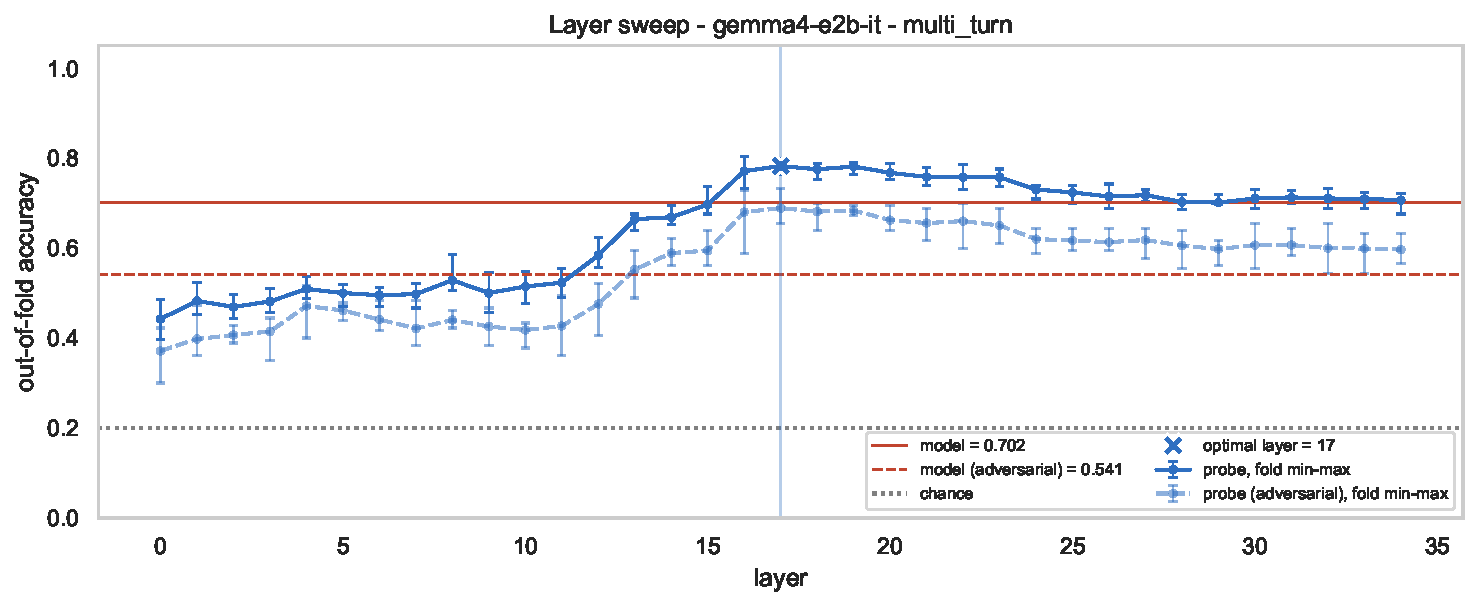
\includegraphics[width=0.85\textwidth]{images/models/gemma4-e2b-it_multi_turn_layers.pdf}
    \caption[Layer sweep, gemma4-e2b-it, multi-turn]{Layer sweep, gemma4-e2b-it, multi-turn.}
    \label{fig:appendix-gemma4-e2b-it-multi-layers}
\end{figure}

\section{Qwen3 4B Instruct 2507}
\label{sec:appendix-layer-sweep-qwen3-4b}

\begin{figure}[H]
    \centering
    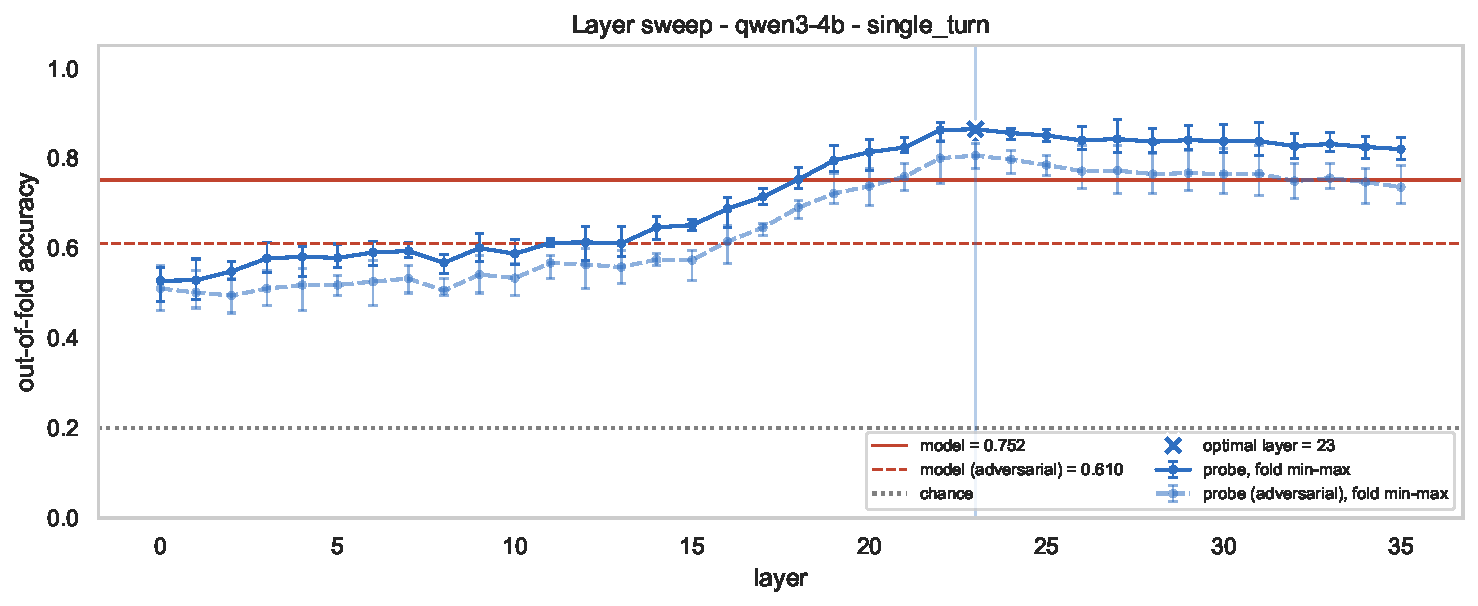
\includegraphics[width=0.85\textwidth]{images/models/qwen3-4b_single_turn_layers.pdf}
    \caption[Layer sweep, qwen3-4b, single-turn]{Layer sweep, qwen3-4b, single-turn.}
    \label{fig:appendix-qwen3-4b-single-layers}
\end{figure}

\begin{figure}[H]
    \centering
    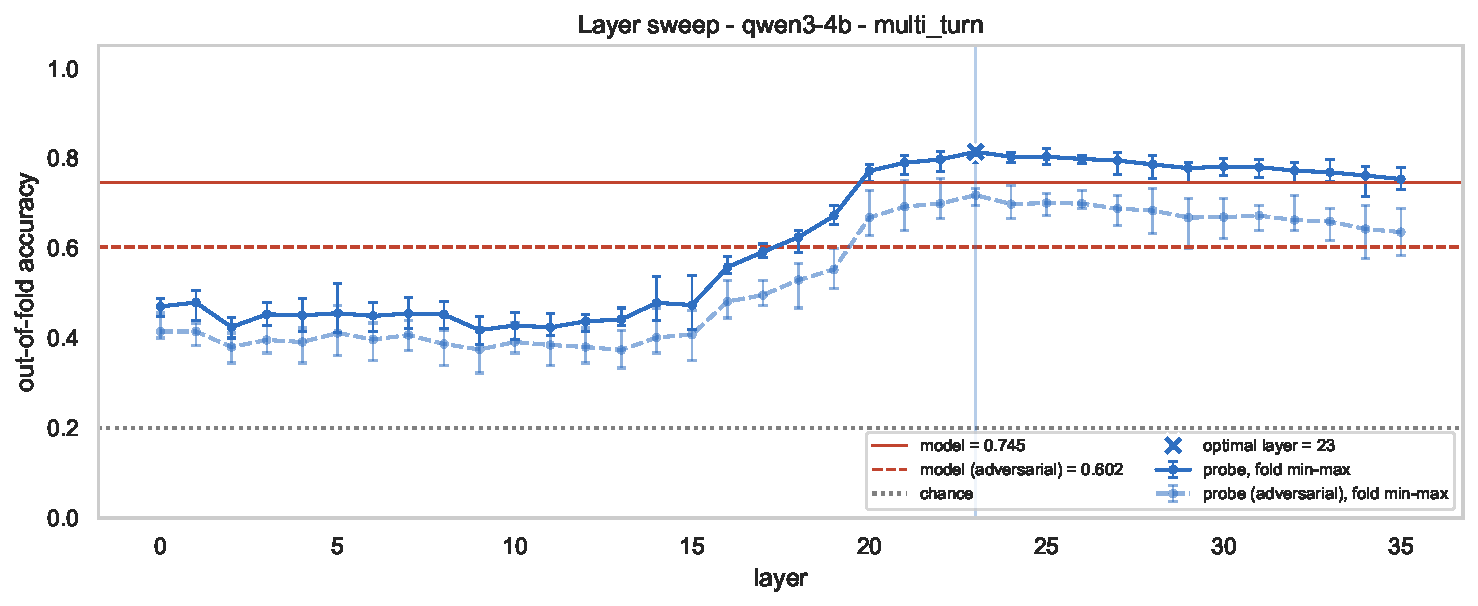
\includegraphics[width=0.85\textwidth]{images/models/qwen3-4b_multi_turn_layers.pdf}
    \caption[Layer sweep, qwen3-4b, multi-turn]{Layer sweep, qwen3-4b, multi-turn.}
    \label{fig:appendix-qwen3-4b-multi-layers}
\end{figure}

\section{Qwen3 8B}
\label{sec:appendix-layer-sweep-qwen3-8b}

\begin{figure}[H]
    \centering
    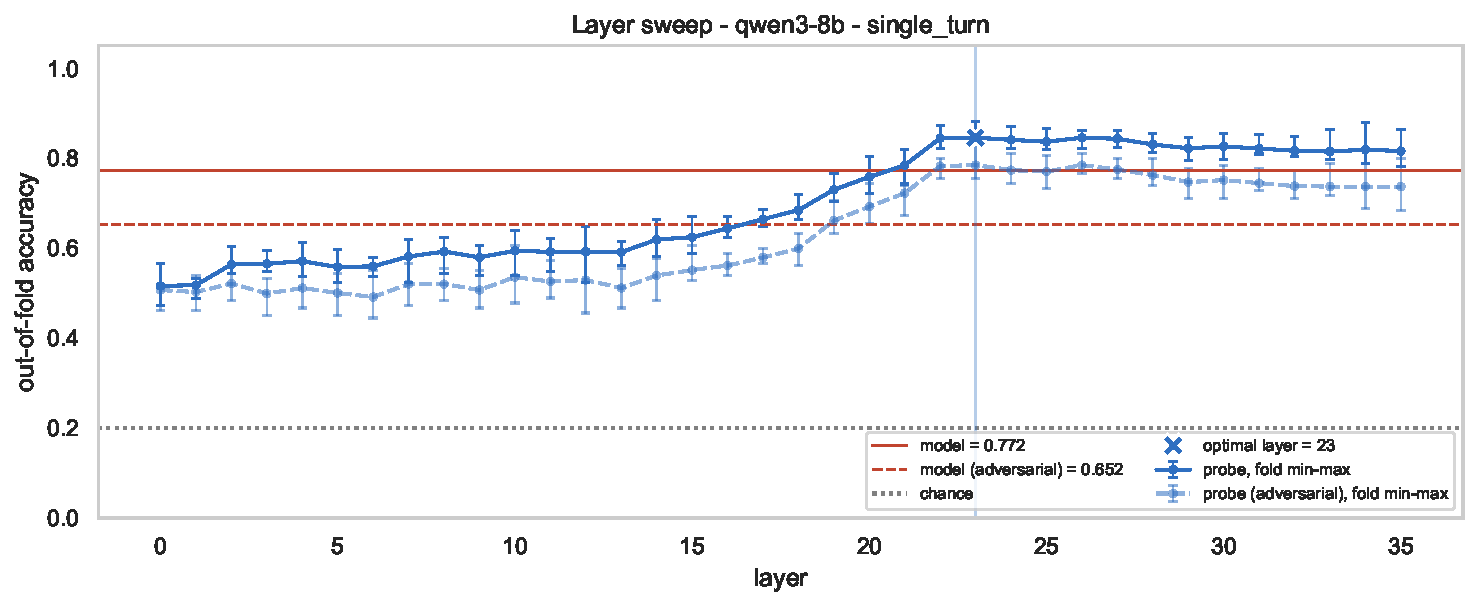
\includegraphics[width=0.85\textwidth]{images/models/qwen3-8b_single_turn_layers.pdf}
    \caption[Layer sweep, qwen3-8b, single-turn]{Layer sweep, qwen3-8b, single-turn.}
    \label{fig:appendix-qwen3-8b-single-layers}
\end{figure}

\begin{figure}[H]
    \centering
    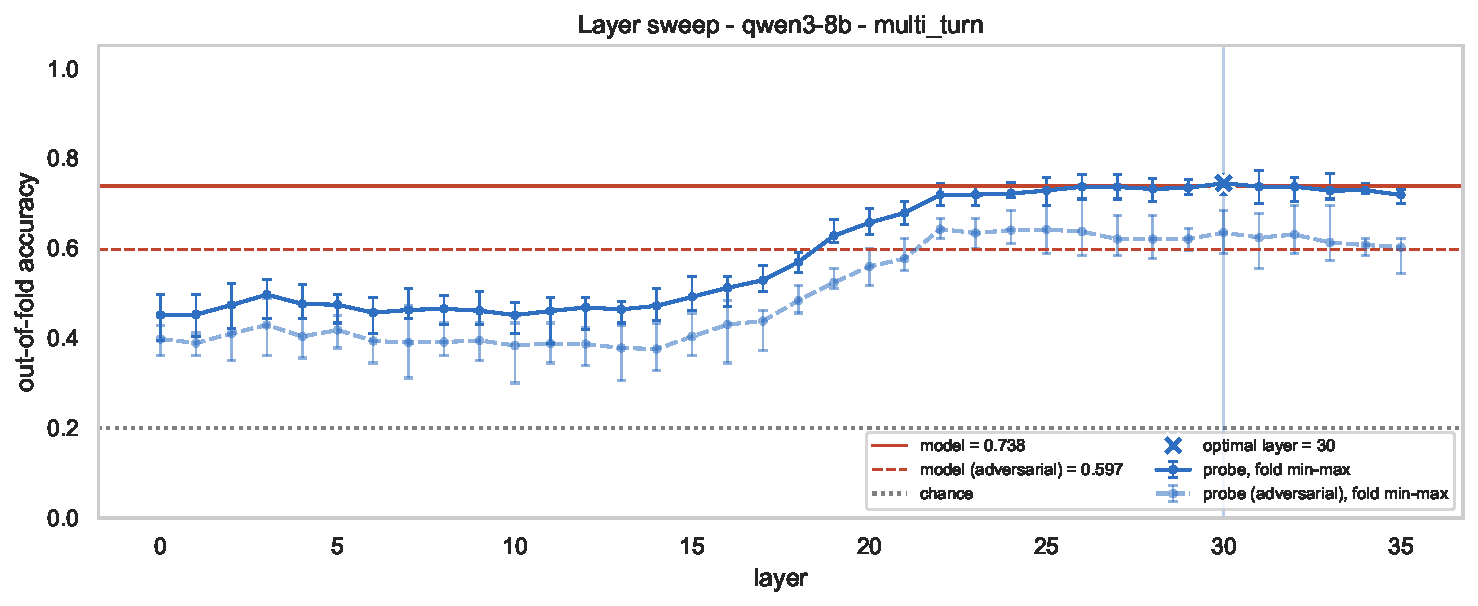
\includegraphics[width=0.85\textwidth]{images/models/qwen3-8b_multi_turn_layers.pdf}
    \caption[Layer sweep, qwen3-8b, multi-turn]{Layer sweep, qwen3-8b, multi-turn.}
    \label{fig:appendix-qwen3-8b-multi-layers}
\end{figure}

\section{Gemma 4 12B IT}
\label{sec:appendix-layer-sweep-gemma4-12b-it}

\begin{figure}[H]
    \centering
    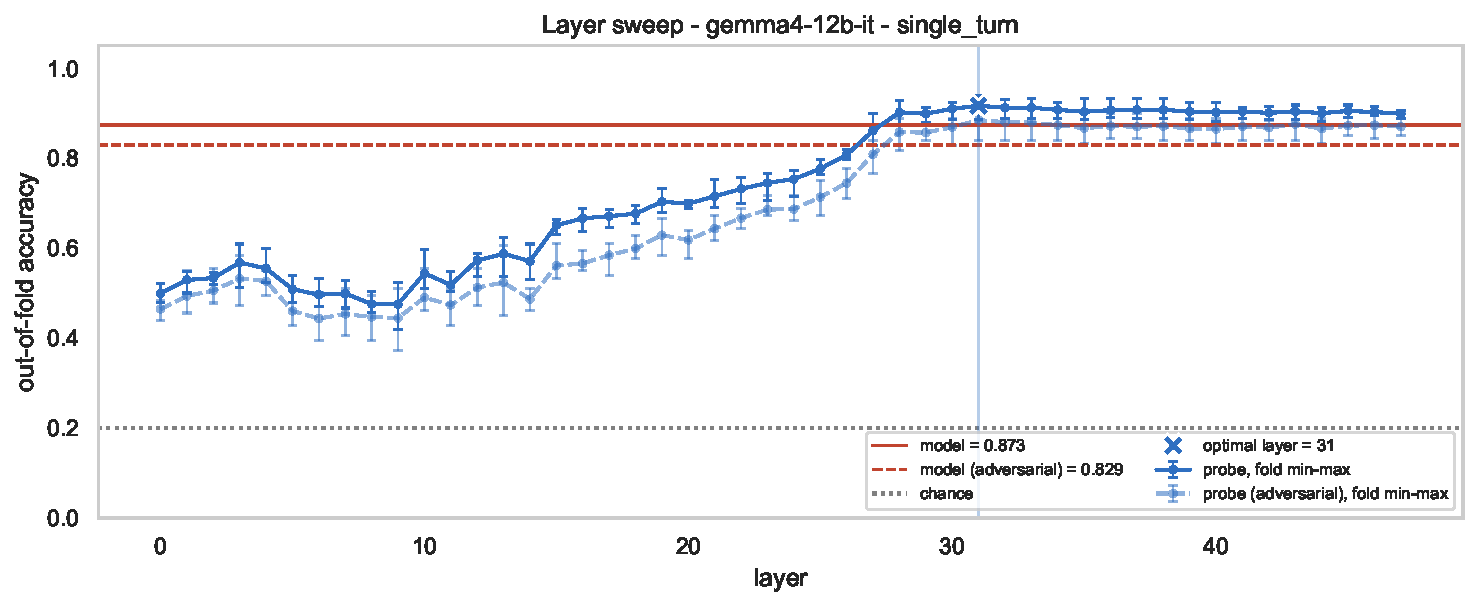
\includegraphics[width=0.85\textwidth]{images/models/gemma4-12b-it_single_turn_layers.pdf}
    \caption[Layer sweep, gemma4-12b-it, single-turn]{Layer sweep, gemma4-12b-it, single-turn.}
    \label{fig:appendix-gemma4-12b-it-single-layers}
\end{figure}

\begin{figure}[H]
    \centering
    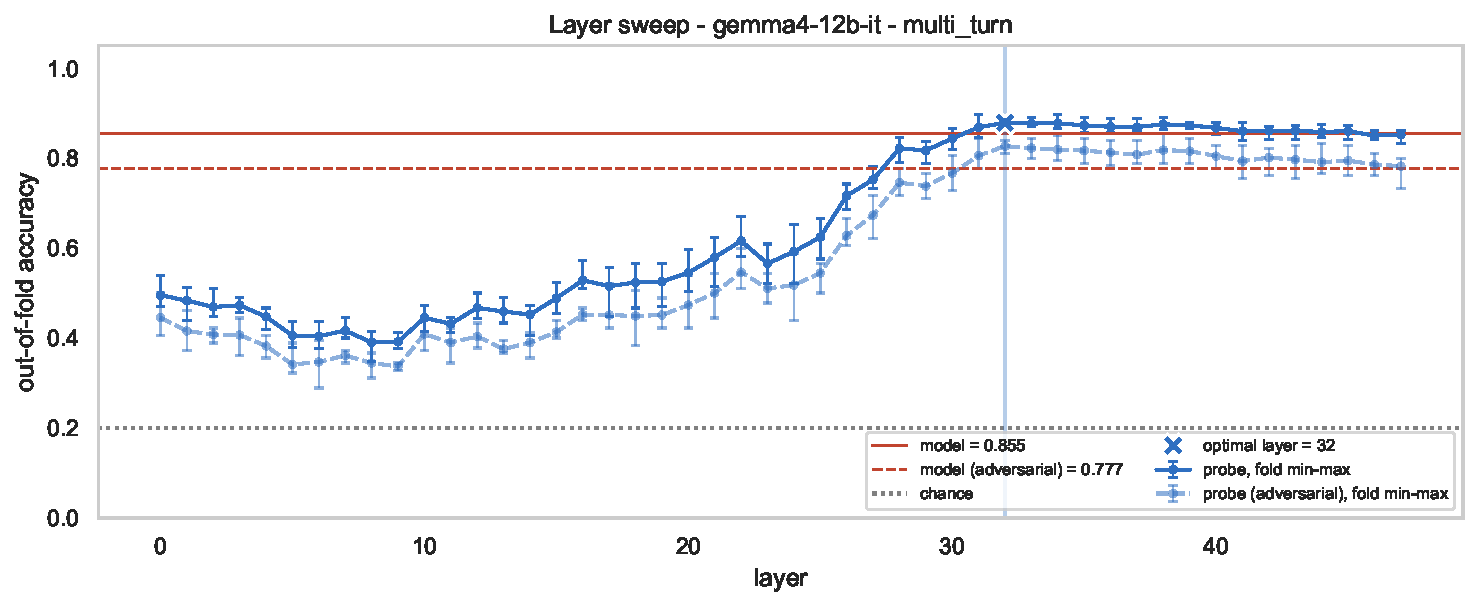
\includegraphics[width=0.85\textwidth]{images/models/gemma4-12b-it_multi_turn_layers.pdf}
    \caption[Layer sweep, gemma4-12b-it, multi-turn]{Layer sweep, gemma4-12b-it, multi-turn.}
    \label{fig:appendix-gemma4-12b-it-multi-layers}
\end{figure}

\section{Gemma 4 26B A4B IT}
\label{sec:appendix-layer-sweep-gemma4-26b-a4b-it}

\begin{figure}[H]
    \centering
    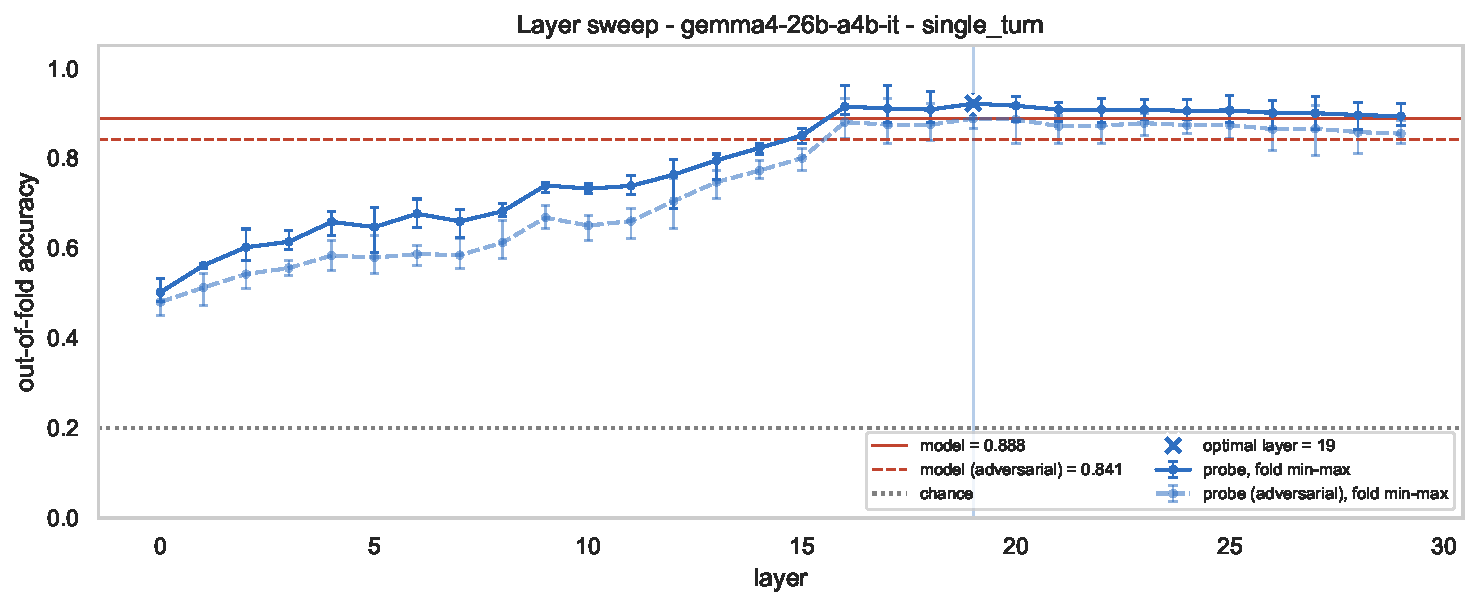
\includegraphics[width=0.85\textwidth]{images/models/gemma4-26b-a4b-it_single_turn_layers.pdf}
    \caption[Layer sweep, gemma4-26b-a4b-it, single-turn]{Layer sweep, gemma4-26b-a4b-it, single-turn.}
    \label{fig:appendix-gemma4-26b-a4b-it-single-layers}
\end{figure}

\begin{figure}[H]
    \centering
    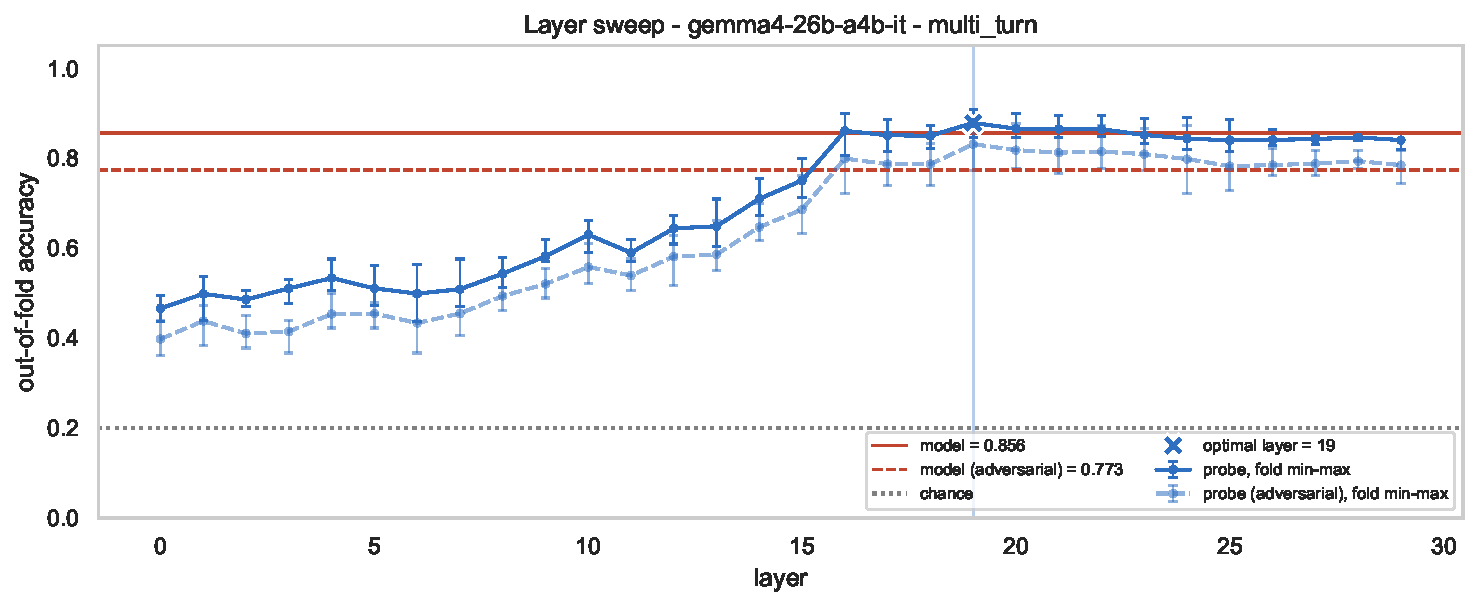
\includegraphics[width=0.85\textwidth]{images/models/gemma4-26b-a4b-it_multi_turn_layers.pdf}
    \caption[Layer sweep, gemma4-26b-a4b-it, multi-turn]{Layer sweep, gemma4-26b-a4b-it, multi-turn.}
    \label{fig:appendix-gemma4-26b-a4b-it-multi-layers}
\end{figure}

\section{Llama 3.3 70B Instruct}
\label{sec:appendix-layer-sweep-llama33-70b}

\begin{figure}[H]
    \centering
    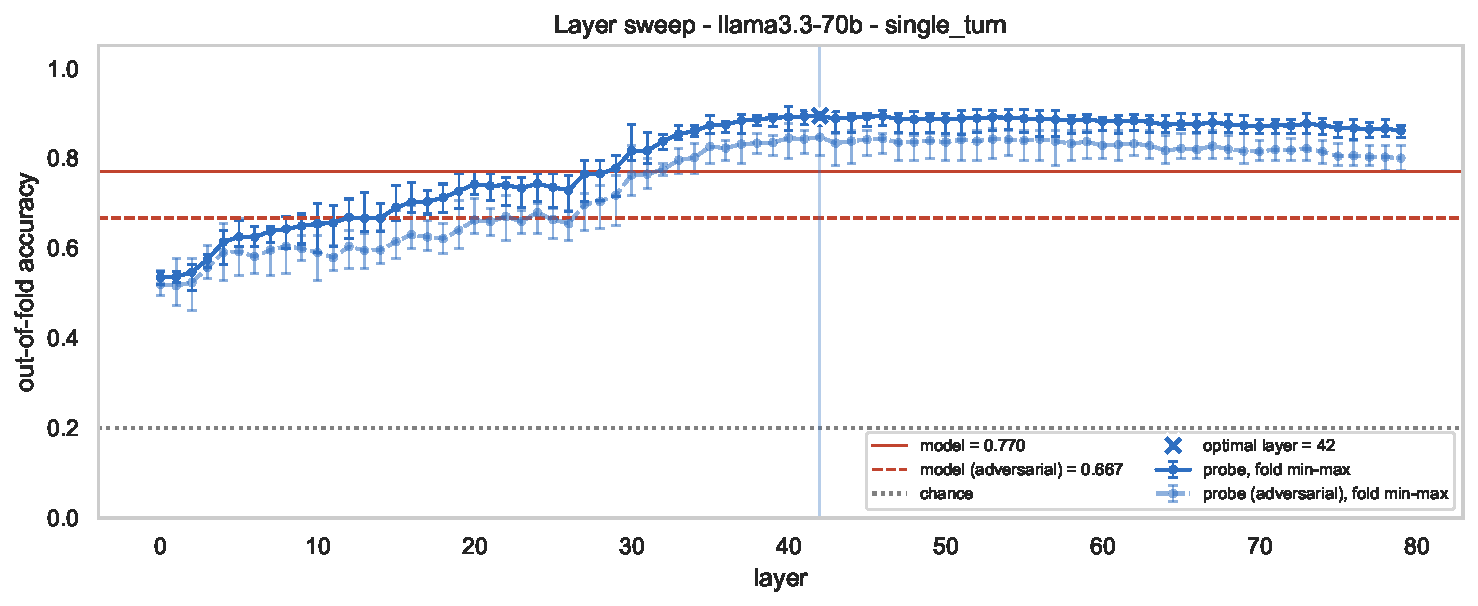
\includegraphics[width=0.85\textwidth]{images/models/llama33-70b_single_turn_layers.pdf}
    \caption[Layer sweep, llama3.3-70b, single-turn]{Layer sweep, llama3.3-70b, single-turn.}
    \label{fig:appendix-llama33-70b-single-layers}
\end{figure}

\begin{figure}[H]
    \centering
    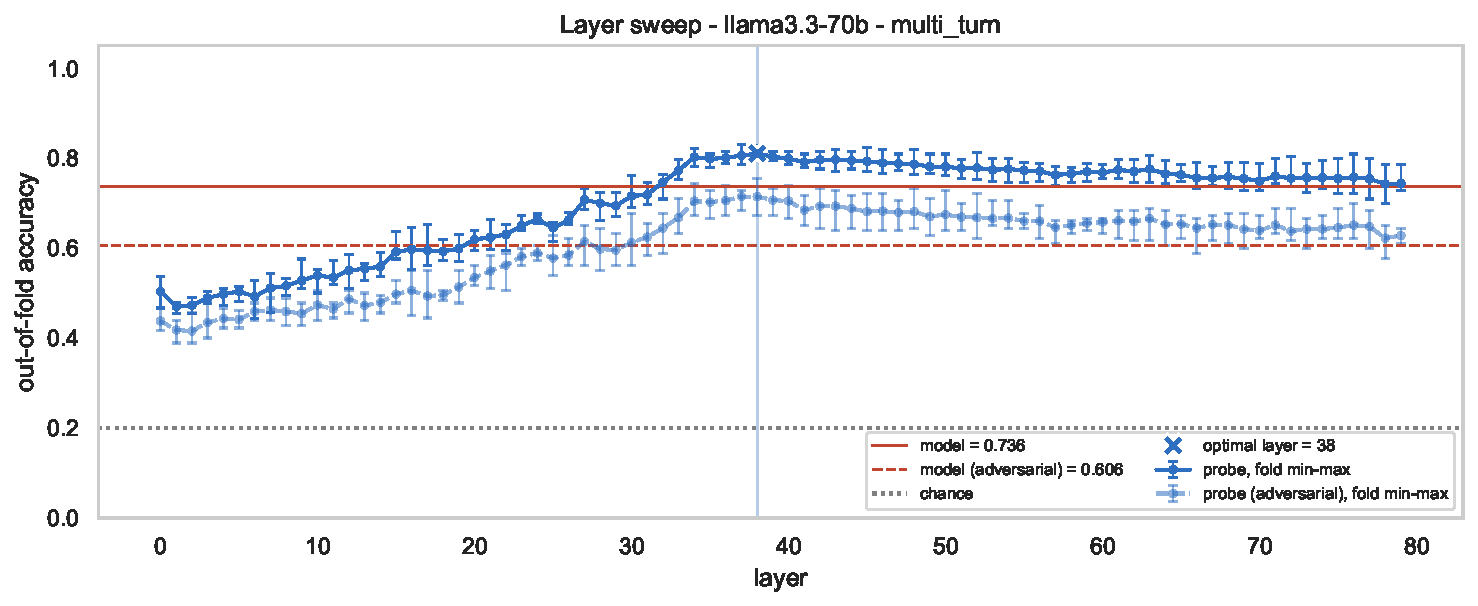
\includegraphics[width=0.85\textwidth]{images/models/llama33-70b_multi_turn_layers.pdf}
    \caption[Layer sweep, llama3.3-70b, multi-turn]{Layer sweep, llama3.3-70b, multi-turn.}
    \label{fig:appendix-llama33-70b-multi-layers}
\end{figure}

\section{Qwen2.5 72B Instruct}
\label{sec:appendix-layer-sweep-qwen25-72b}

\begin{figure}[H]
    \centering
    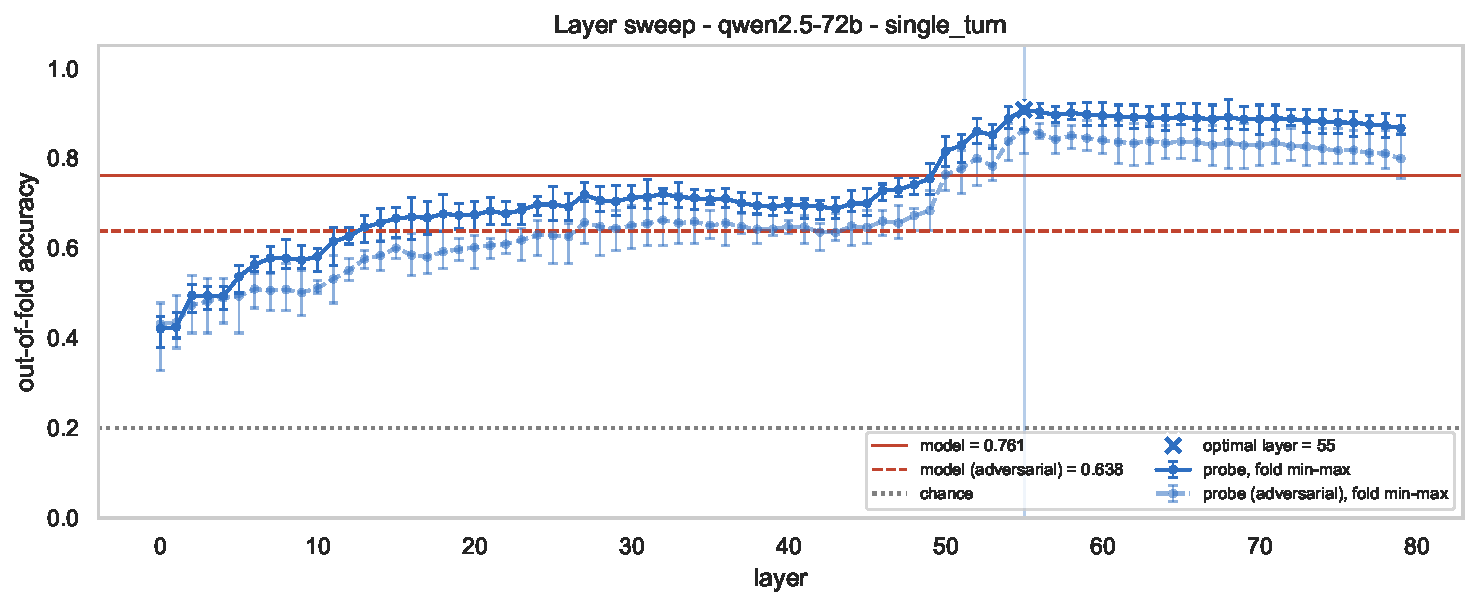
\includegraphics[width=0.85\textwidth]{images/models/qwen25-72b_single_turn_layers.pdf}
    \caption[Layer sweep, qwen2.5-72b, single-turn]{Layer sweep, qwen2.5-72b, single-turn.}
    \label{fig:appendix-qwen25-72b-single-layers}
\end{figure}

\begin{figure}[H]
    \centering
    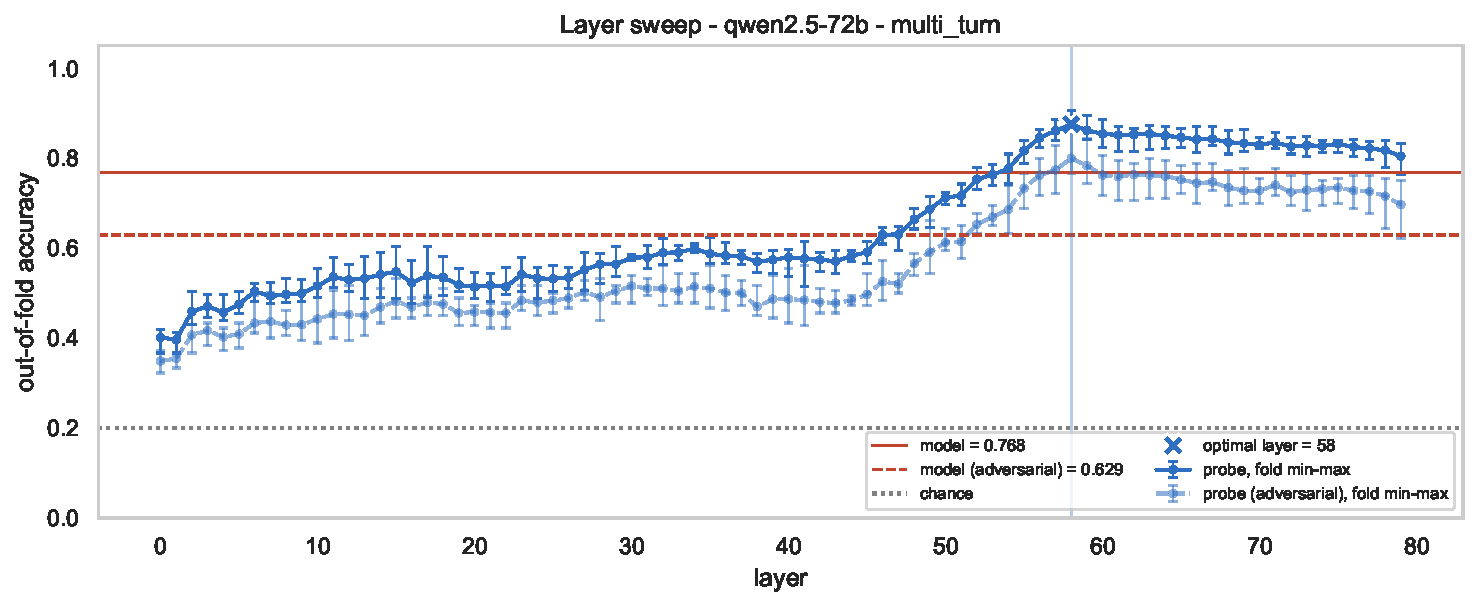
\includegraphics[width=0.85\textwidth]{images/models/qwen25-72b_multi_turn_layers.pdf}
    \caption[Layer sweep, qwen2.5-72b, multi-turn]{Layer sweep, qwen2.5-72b, multi-turn.}
    \label{fig:appendix-qwen25-72b-multi-layers}
\end{figure}

\section{GPT-OSS 20B}
\label{sec:appendix-layer-sweep-gpt-oss-20b}

\begin{figure}[H]
    \centering
    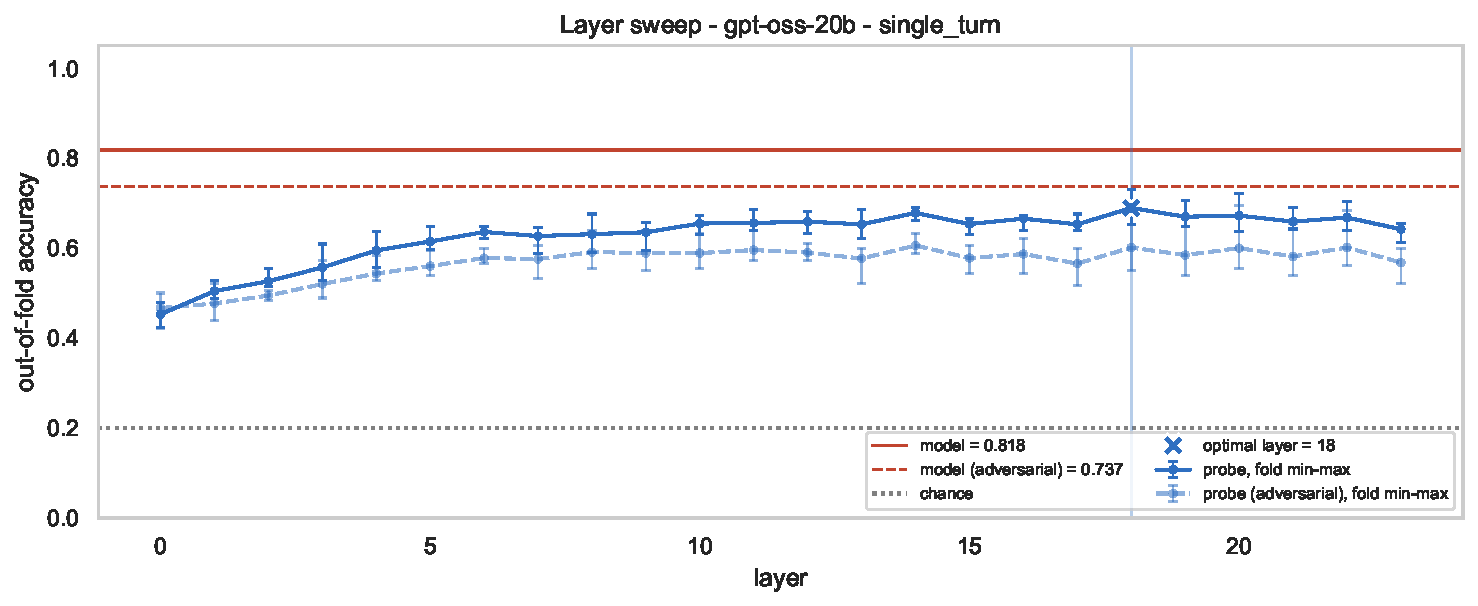
\includegraphics[width=0.85\textwidth]{images/models/gpt-oss-20b_single_turn_layers.pdf}
    \caption[Layer sweep, gpt-oss-20b, single-turn]{Layer sweep, gpt-oss-20b, single-turn.}
    \label{fig:appendix-gpt-oss-20b-single-layers}
\end{figure}

\begin{figure}[H]
    \centering
    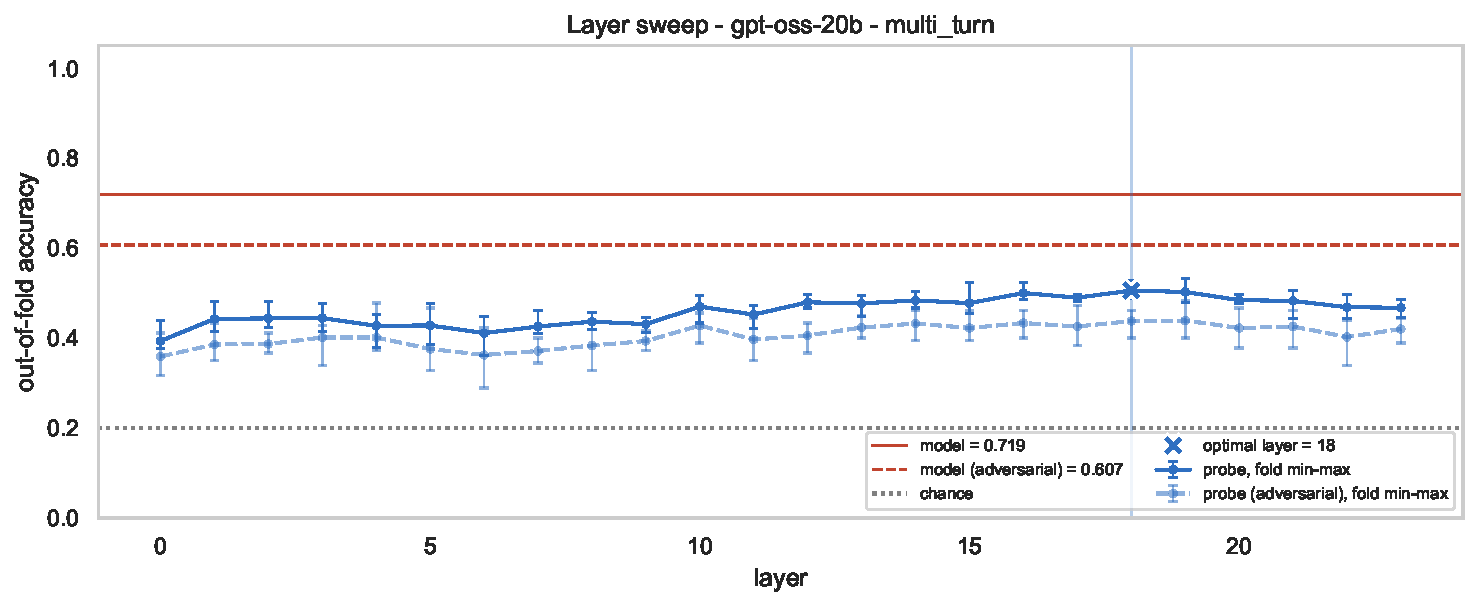
\includegraphics[width=0.85\textwidth]{images/models/gpt-oss-20b_multi_turn_layers.pdf}
    \caption[Layer sweep, gpt-oss-20b, multi-turn]{Layer sweep, gpt-oss-20b, multi-turn.}
    \label{fig:appendix-gpt-oss-20b-multi-layers}
\end{figure}

\begin{figure}[H]
    \centering
    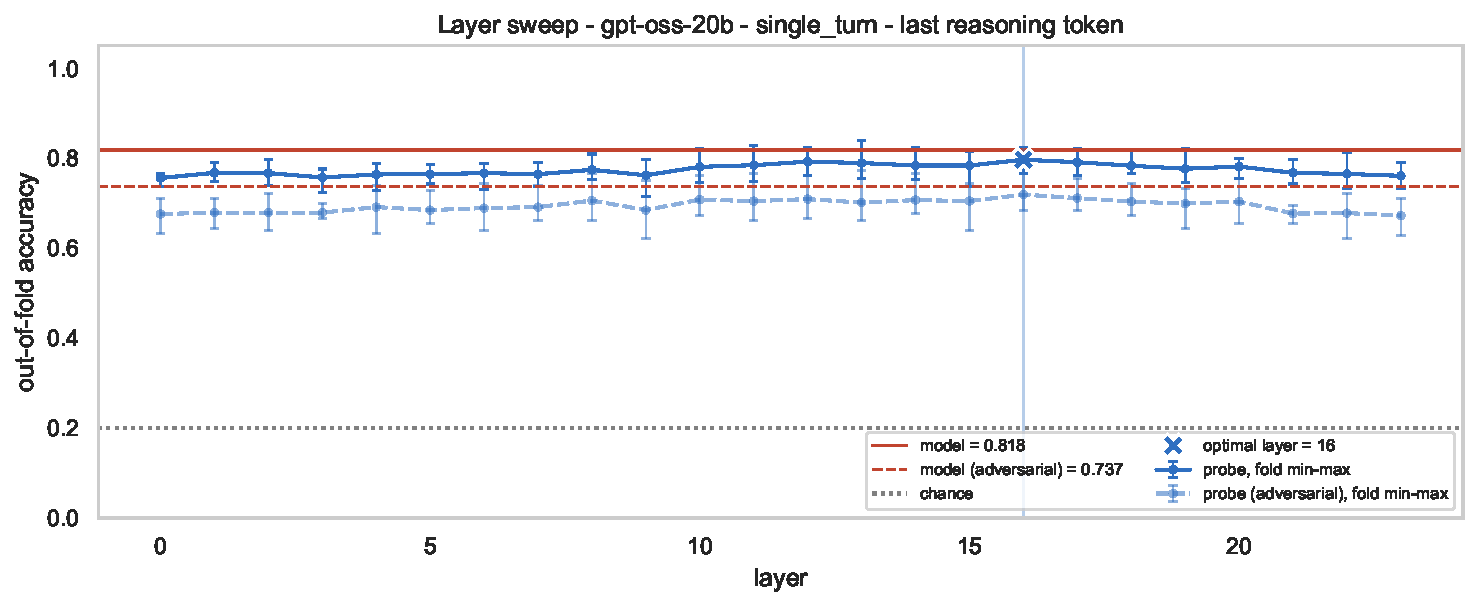
\includegraphics[width=0.85\textwidth]{images/models/gpt-oss-20b_single_turn_reasoning_layers.pdf}
    \caption[Layer sweep, gpt-oss-20b, single-turn, last reasoning token]{Layer sweep, gpt-oss-20b, single-turn, hidden states at the last reasoning token (Section~\ref{subsec:ch8-gpt-oss-reasoning}).}
    \label{fig:appendix-gpt-oss-20b-single-reasoning-layers}
\end{figure}
